\chapter{Implementing the System: The Front-End}
	In chapter \ref{chap:impl:backend} the implementation of the back-end was described. In this section, the implementation of the corresponding front-end will be described. It is implemented following the design specifications from chapter \ref{chap:design}.

	\section{Developing for the Browser}
		When developing for the browser, there are three ``possibilities'': JavaScript, Java applets, and Flash. However, from a technological point of view, Flash is horribly outdated. The usage of the Flash plugin has simply declined so much, that it is no longer feasible. Using Java applets are, similarly to Flash, simply outdated. Introducing too many security concerns, issues, and cross-platform issues, this is simply not a good choice.

		This leaves us with JavaScript. This \emph{is} the language that pretty much all interactive web applications are developed today. As such, it is what will be used for this project.


	\section{Using a Framework}
		While it would be possible to develop projects using nothing but ``pure'' JavaScript, it seems hardly worth it, re-inventing the wheel. After all, a solid framework will greatly aid in the development of the project. Of the more popular front-end frameworks, the following can be mentioned:
		\begin{itemize}
			\item Angular 1.5/2.0
			\item ReactJS
			\item Ember
			\item Backbone
		\end{itemize}
		Choosing the ``right'' framework, is a very subjective thing: There are pros and cons with each of the choices. However, Angular is without a doubt the \emph{largest} project. As such, there are more third party packages available, which will speed up development. Consequently, there are also significantly more resources available in regards to achieving certain goals in regards to functionality. As such, it is chosen that Angular will be the framework for this project.


		\subsection{A Framework for the Framework}
			All is not said and done, however. Angular comes in two variants: Angular 1.5, which is tried and tested, and Angular 2.0 which is still in beta. Angular 2.0 focuses a lot more on web-components, than Angular 1.5, and as such, it will most likely generate more re-usable code. 

			But this is not everything. Most modern web applications uses a framework for the graphical interface as well. Projects as Bootstrap has revolutionized the way these applications are developed. Recently, contenders for the place as the go-to graphical framework, has popped up. Most noticeably Angular Material, by Google. Angular Material supports Angular \emph{natively}. There are UI bindings available for \emph{all} components. Bootstrap, on the other hand, requires third party bindings. 

			Finally, there is the concept of responsive web design. One of the biggest arguments for developing a web UI \emph{(see section \ref{sec:design:frontend}, on page \pageref{sec:design:frontend})}, was that it would give a similar experience across multiple platforms. After a brief examination of the two frameworks, it is found that Angular Material does this significantly easier, using their flexboxes. This ensures that the websites components are re-arranged according to the screen size of the device browsing the web application.

			\emph{However}, Angular Material \emph{only} supports Angular 1.5. As such, it is determined that the project will use Angular 1.5 with the Angular Material UI framework.

	\section{Being Responsive}
		When it comes to developing websites and web applications, one of the most important aspect is responsiveness. In short, it is defined as a website that behaves accordingly to the available screen area. This is without a doubt one of Angular Material's strengths. The best example of this responsiveness, is the main interface's menu, on the right side. This is seen on figures \ref{fig:impl:responsive:locked} to \ref{fig:impl:responsive:expanded} on page \pageref{fig:impl:responsive:locked}. Figure \ref{fig:impl:responsive:locked} shows the side menu being locked open, since the screen is large enough to allow this. Figure \ref{fig:impl:responsive:collapsed} shows the side menu in its collapsed form. Clicking the standard Material Design expand icon, in the upper left corner will expand the menu, the result of which is seen on figure \ref{fig:impl:responsive:expanded}.

		\begin{figure}
			\centering
			\begin{subfigure}[b]{0.75\textwidth}
				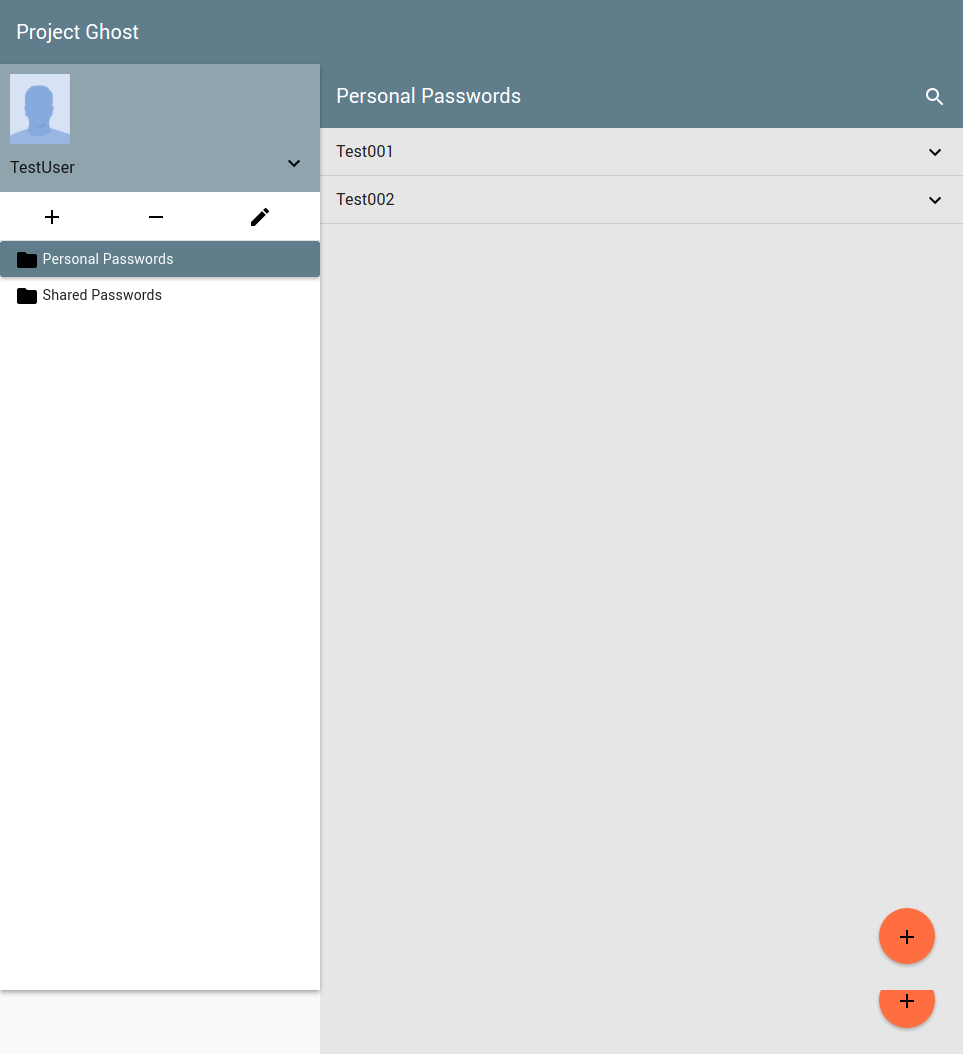
\includegraphics[width=\linewidth,clip,trim=0 800 200 0]{figures/implementation/screenshots/ghost_main_locked_menu.png}
				\caption{Main interface with the side menu locked in open position, due to plenty of screen space.}
				\label{fig:impl:responsive:locked}
			\end{subfigure}

			\begin{subfigure}[b]{0.75\textwidth}
				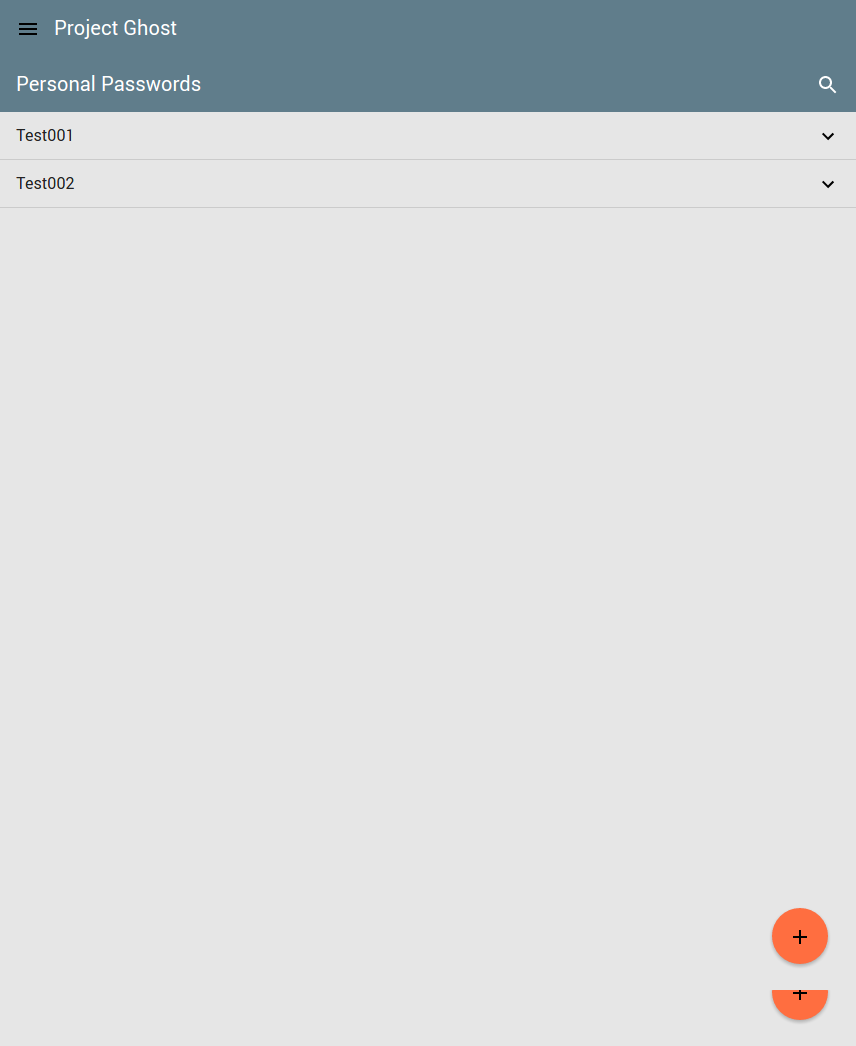
\includegraphics[width=\linewidth,clip,trim=0 800 200 0]{figures/implementation/screenshots/ghost_main_collapsed_menu.png}
				\caption{Main interface with the side menu collapsed, due to lack of screen space.}
				\label{fig:impl:responsive:collapsed}
			\end{subfigure}

			\begin{subfigure}[b]{0.75\textwidth}
				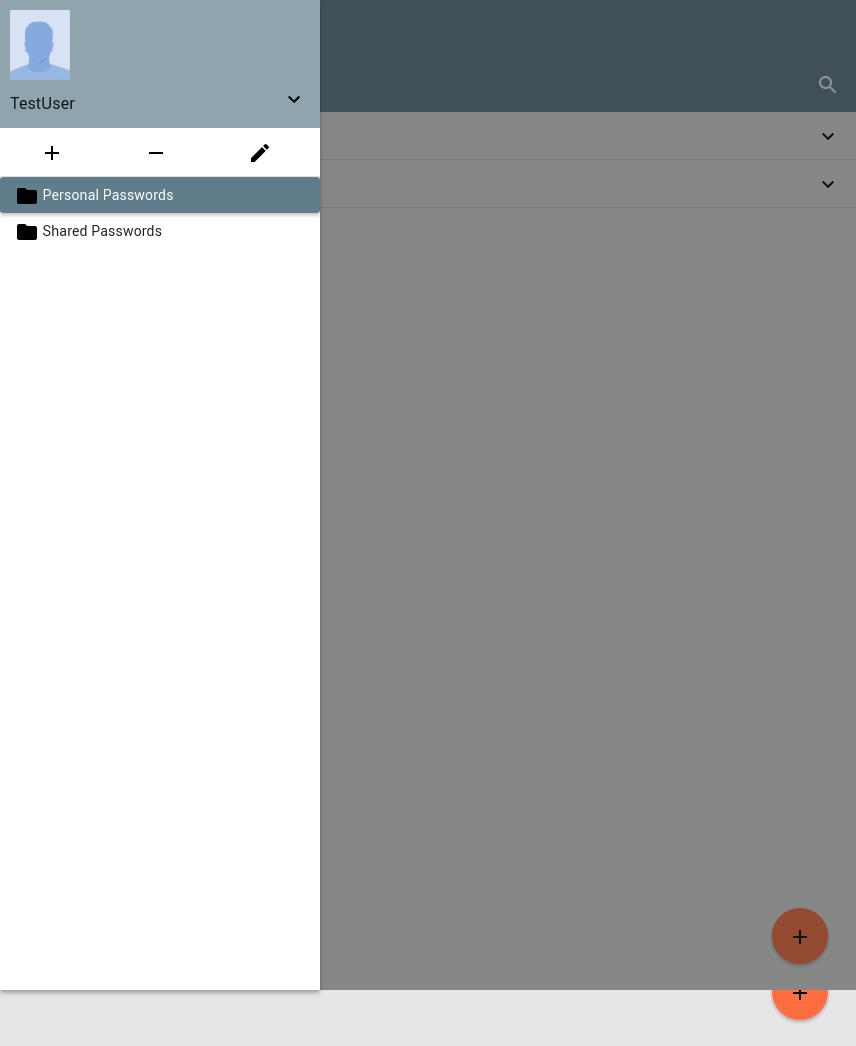
\includegraphics[width=\linewidth,clip,trim=0 800 200 0]{figures/implementation/screenshots/ghost_main_expanded_menu.png}
				\caption{Main interface with the side menu expanded, in order for the user to access it.}
				\label{fig:impl:responsive:expanded}
			\end{subfigure}

		\end{figure}

	\section{Structuring the Codebase}
		In section \ref{sec:impl:backend:codebase} on page \pageref{sec:impl:backend:codebase} the importance of a properly structured codebase, was argued for. 

		Angular is -- for better or worse -- a very \emph{opinionated} framework. This means that there exists very particular guides, as to how Angular applications should be made and structured. One of the most popular guides to this, is John Papa's Angular 1 Style Guide\cite{johnpapa_angular1}.

		He suggests that the best structure, is a ``group by feature''-structure. In this context, it would for instance mean that the login page and controller are located in the same folder. The same would then go for the password creation page, etc.

		Naming the files in said feature folders, is then rather simple. The feature name is simply appended by the type of contents, inside of said file. These types are primarily:
		\begin{enumerate}
			\item Template
			\item Controller
			\item Service
		\end{enumerate}
		As such, using login and password as an example, the structure will look as follows. While this \emph{definitely} is not all of the front-end's files, it goes show the point: It is very neatly organized, and files which are related are found right next to eachother.

		\dirtree{%
		.1 app.
		.2 index.html.
		.2 login.
		.3 login.template.html.
		.3 login.controller.js.
		.2 password.
		.3 password.template.html.
		.3 password.controller.js.
		}

	\section{Encryption \& Hashing}
		While in theory one could go about implementing the algorithms needed for the implementations oneself, the fact is that this would both be \emph{way} too resource demanding, and it would also introduce security risks, in forms of implementational errors. As such, it is chosen to go with an encryption library, which will handle the encryption.

		For this purpose, the Forge library is chosen\cite{forge-encryption}. Forge is a collection of encryption algorithms, developed in pure JavaScript and is as such able to be executed in the browser directly. In its suite of encryption algorithm is not only AES, but also RSA key \emph{generation} and \emph{encryption}. As such, it alone houses all of the required cryptographic tools, to develop the front-end of the solution.

		\subsection{Deviating From the Designs}
			Unfortunately, the implementation must \emph{deviate} from the designs. Seeing as Argon2 only exists as a C++ implementation, it is simply not able to be executed in the browser. As such, it is \emph{unfortunately} necessary to choose another key derivation function, in accordance with section \ref{sec:kdf}, on page \pageref{sec:kdf}. Seeing as Forge actually contains an implementation of PBKDF2, this is chosen as the tool for deriving the encryption key. This choice is highly based upon interoperability, as the output from one algorithm will be guaranteed to work with the other.

	\section{Generating Passwords}
		One, until now, overlooked part, is password \emph{generation}. Since the solution aims at giving users the ability to use complex and ``strong'' passwords, it only makes sense that the solution can actually \emph{generate} these passwords.

		First and foremost, it is important to give the user the ability to customize the length of the password. Unfortunately, some systems only supports passwords of a certain length. Then there is the matter of which symbols that the password consists of. The UI for this is seen on figure \ref{fig:impl:password:generate}, on page \pageref{fig:impl:password:generate}. However, the interesting part is the code that powers it.

		Following the Angular style, it is powered by an \verb=PasswordGeneratorService=. This has two functions -- no more. The first generate a so-called table. It is from this table, that the final password will be generated. The method really does nothing more then concatenate four arrays of characters, depending on the selections the user made from figure \ref{fig:impl:password:generate}.

		Once the table has been created, it is time for the \emph{actual} password to be generated. This is the critical part of the code. Should the password generator end up being biased, it would make it easier for attackers to bruteforce passwords, they know to be generated by this solution. As such, a \emph{secure} random is used, from the forge library. While this method most likely was not supposed to be used outside their own library, it serves this purpose quite well. \emph{However}, this generates a random \emph{byte} -- i.e. a number between $0$ and $255$.

		There are now two options. Either the generated table is ``stretched'' to fit 255 characters, or the value is scaled down to fit the length of the table. Imagine the user having selected lower case letters, upper case letters, and digits -- a fairly common requirement for passwords. This results in $26$ lower case letters, $26$ upper case letters, and $10$ digits \emph{(assuming it is the English alphabet that is used)}. This totals at $62$ characters.

		Should it be chosen to stretch this, it would mean repeating the table, until $255$ characters are used. As such, a pattern will emerge:
		\begin{verbatim}
			'a','b','c','d','e','f','g','h','i','j','k','l','m','n','o','p','q',
			'r','s','t','u','v','w','x','y','z','A','B','C','D','E','F','G','H',
			'I','J','K','L','M','N','O','P','Q','R','S','T','U','V','W','X','Y',
			'Z','0', '1', '2', '3', '4', '5', '6', '7','8', '9','a','b','c','d',
			...................................................................,
			'a','b','c','d','e','f','g','h'
		\end{verbatim}
		While most of the characters \emph{would} be represented an equal amount of times, the characters \verb=a= through \verb=h= will \emph{not}. This is simply due to $256\%62=8$, and as such the first $8$ characters will be represented \emph{once} more, than the remaining $54$. The approach is, what is called biased. As such, it is \emph{not} the preferable way to do this.

		The other approach is to simply limit the byte value, to a number between $0$ and $61$ \emph{($62-1$, JavaScript is zero-indexed)}. The \emph{simplest} approach to this, is simply disregard \emph{any} values of $62$ or above. After all, if it is known that the secure random is evenly distributed between the values $0$ and $255$, simply ignoring values of $62$ and above, \emph{should} result in evenly distribution amongst values $0$ through $61$. 

		There is one caveat with this approach, however. Since they're \emph{random} numbers, it is unfortunately not possible to 100\% guarantee termination of the algorithm. In the trials performed until now, this has not been an issue. However, should this become an issue a simple limit to the about of tries before failing can be introduced. When this limit is reached, the algorithm terminates itself, and re-tries. The code for this algorithm -- without the max tries limiter -- is shown on listing \ref{lst:impl:password:generate} on page \pageref{lst:impl:password:generate}


		\begin{figure}[p]
			\centering
			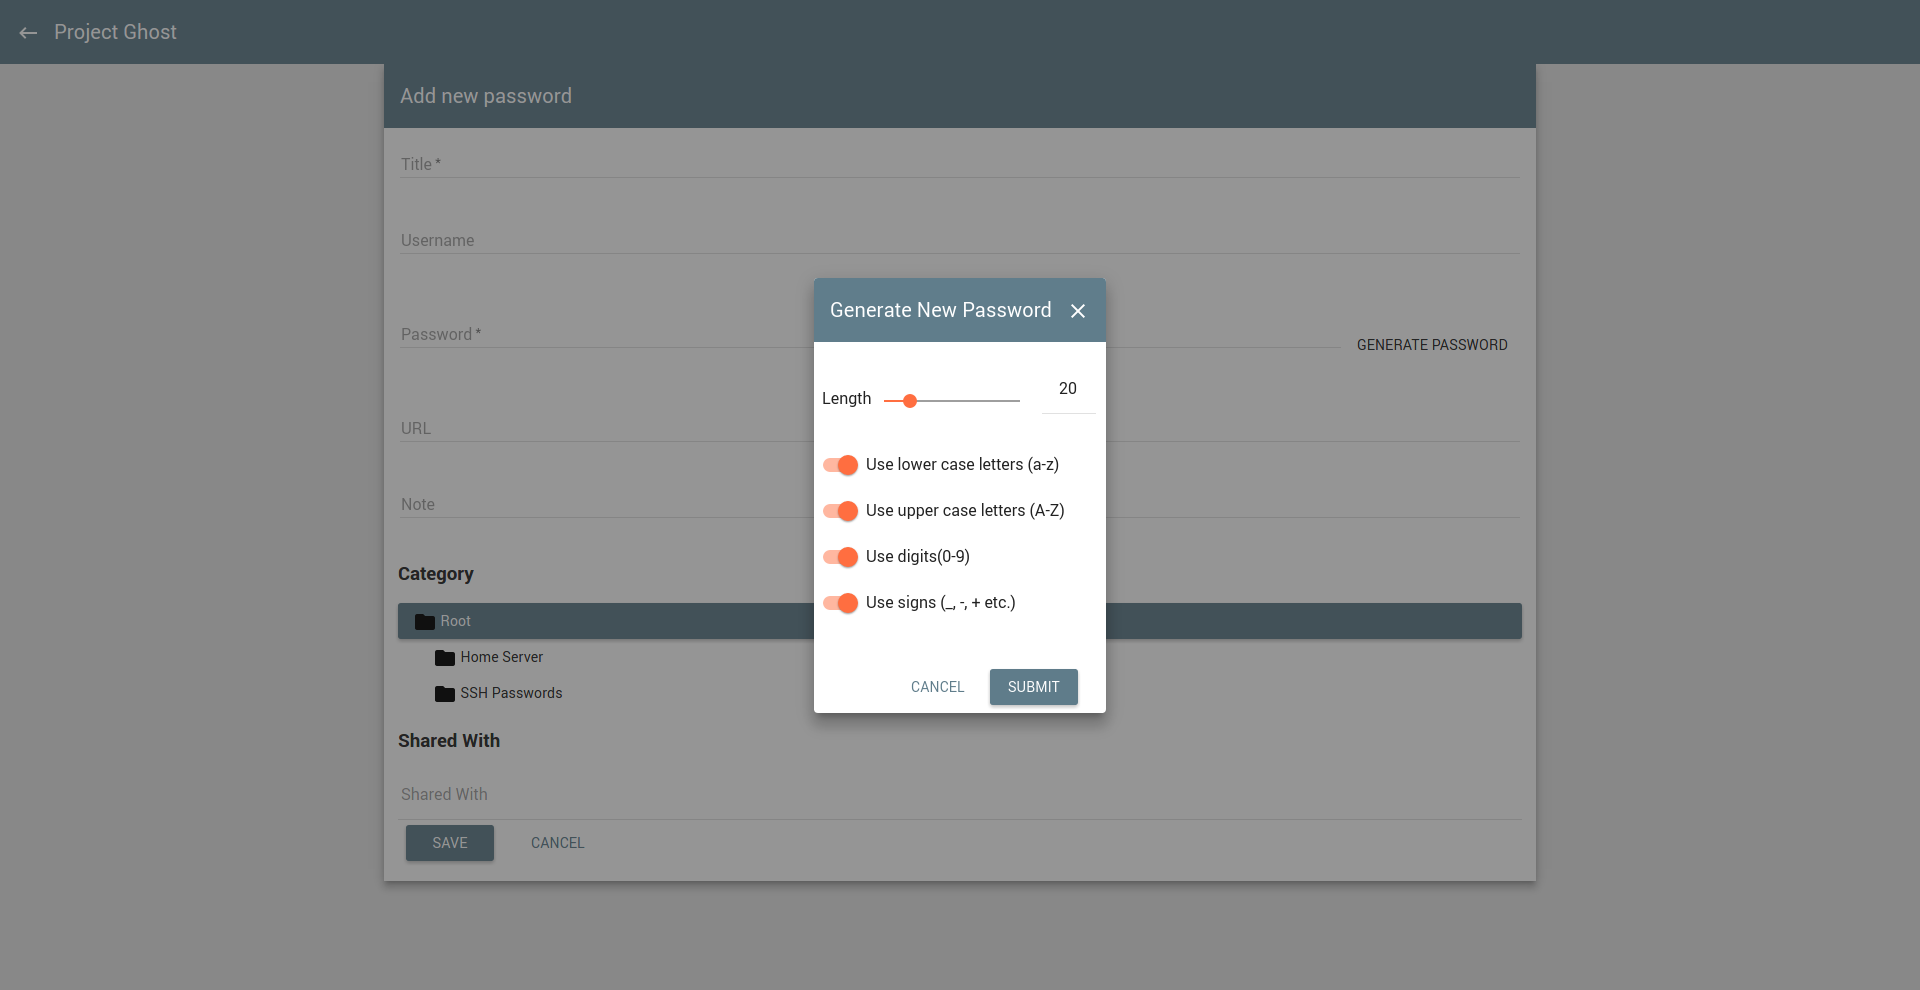
\includegraphics[width=0.4\textwidth,clip,trim=750 250 750 250]{figures/implementation/screenshots/add-password.png}
			\caption{Generating new password.}
			\label{fig:impl:password:generate}
		\end{figure}

		\begin{lstlisting}[language=Javascript,gobble=12,caption={Generating the password, using the value cut-off method},label={lst:impl:password:generate}]
            function generate(characters, length){
                var password = '';
                for( var i = 0 ; i < length ; i++ ){
                    var byte = forge.random.getBytesSync(1);
                    while( byte.charCodeAt(0) >= characters.length ){
                        byte = forge.random.getBytesSync(1);					
                    }
                    password = password + characters[byte.charCodeAt(0)];
                } 
                return password;
            }	
		\end{lstlisting}

	\section{Making A Tree}
		While Angular Material generally is a \emph{very} good graphical framework -- especially taking its relative young age into consideration -- it lacks some things, which is required for the implementation. Specifically, it lacks a tree-like menu, for showing the password categories \emph{(see \ref{sec:model:category} on page \pageref{sec:model:category})}. This is, to a great extent, because the Material Design specification never includes this as an actual component. 

		However, since this \emph{is} required for the project, a custom web component is implemented. At the base of this component, the default Angular Material buttons are used, for a consistent UI. However, certain things are disabled. For instance, the Material Design specifications dictate that buttons' text are to be in upper case. This is not preferable for creating the structures, and as such it is disabled.

		Based in the data from the category models \emph{(see section \ref{sec:model:category})}, a JSON tree can easily be made. An example of this structure is found on listing \ref{lst:frontend:tree:data} on page \pageref{lst:frontend:tree:data}. This data structure will then result in the tree found on figure \ref{lst:frontend:tree:result} on page \pageref{lst:frontend:tree:result}.

		Having said all this, it is never actually explained \emph{how} the structure works. The outer most component is the \verb=tree-menu=. This controls everything. First it loops over each element in the current level. Using the example from listing \ref{lst:frontend:tree:data}, this means the categories with titles ``Title001'' and ``Title002''. For each of these elements, it creates a new \verb=tree-node=. Each of these \verb=tree-node=s then loops over their children, and so forth. Each of these \verb=tree-nodes= are represented as a button, from a graphical point of view.

		In the end, through this recursion, a tree consisting of tree-nodes will be created. They will look as depicted on figure \ref{lst:frontend:tree:result}. Whenever one of the nodes are clicked, it is propagated up through the tree, using references to each node's parents. When this propagation reaches the parent \verb=tree-menu= object, the method specified using its \verb=on-select= directive, is invoked. That way, the controller can determine what happens, when the user clicks each category entry.


		\begin{lstlisting}[style=json2,gobble=12, caption={The front-end's category tree data structure},label={lst:frontend:tree:data}]
            [
                {
                    id: 1,
                    title: 'Title001',
                    children: [
                        {
                            id: 11,
                            title: 'Title001-001',
                            children: []
                        },
                        {
                            id: 12,
                            title : 'Title001-002',
                            children: []
                        }
                    ]
                },
                {
                    id: 2,
                    title: 'Title002',
                    children: []
                }
            ]
		\end{lstlisting}
	
		\begin{figure}[p]
			\centering
			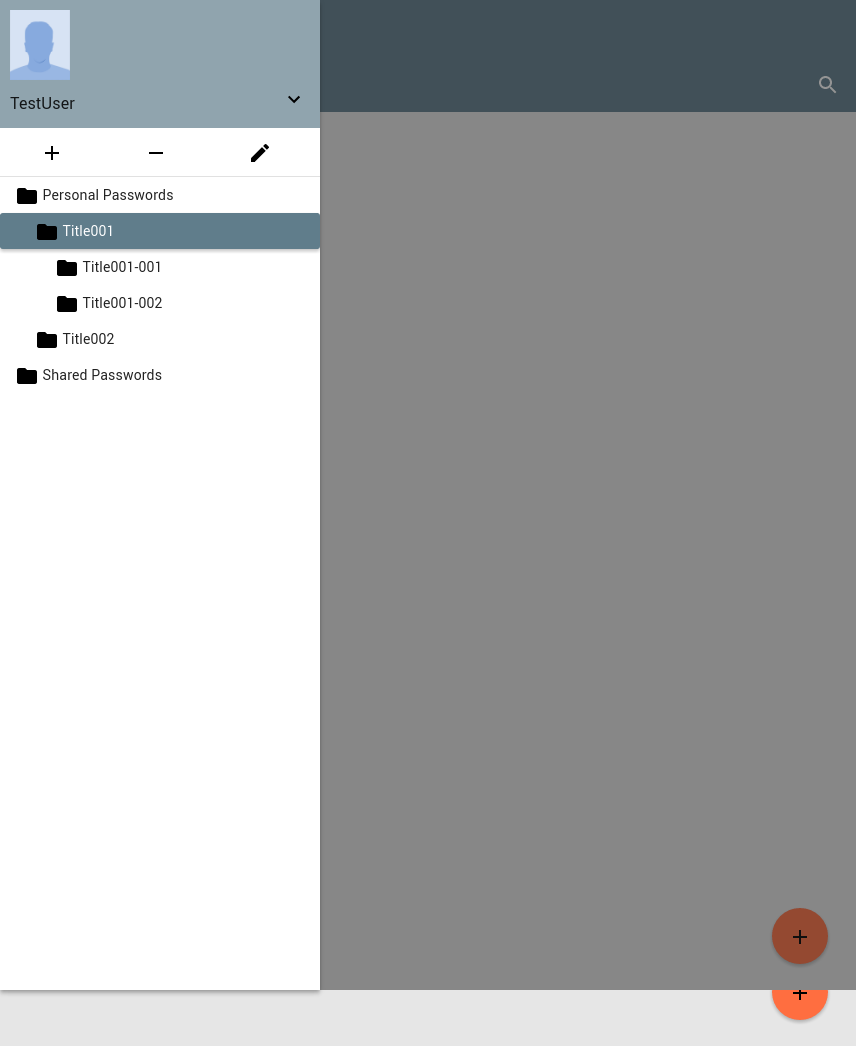
\includegraphics[width=0.8\textwidth,clip,trim=0 690 536 210]{figures/implementation/screenshots/example_tree.png}
			\caption{The resulting tree, of the data specified on figure \ref{lst:frontend:tree:data} on page \pageref{lst:frontend:tree:data}.}
			\label{lst:frontend:tree:result}
		\end{figure}